%
% File: chap04.tex
% Author: Your Name
% Description: Conclusion
%
\let\textcircled=\pgftextcircled
\chapter{Research results}
\label{chap:intro}

\section{Verification of Model Assumptions}
\initial{T}o use the OLS method to estimate the coefficients in linear regression analysis, a number of assumptions must be satisfied. An unbiased estimation of model parameters requires the fulfillment of the Gauss-Markov assumptions (MLR1-MLR4). Furthermore, if MLR1-MLR6 are fulfilled, the OLS estimation is said to be the best linear unbiased estimator (BLUE). 
\\

\textbf{MLR1: Linear in Parameters
}
To detect nonlinearity we inspected plots of residuals vs. predicted values. Points symmetrically distributed around the horizontal line indicate that we do not violate MLR1.
Unfortunately, only the models with employment growth as the dependent variable (models EB, EBI, EIB) validate this assumption. The other models with sales and labor productivity growth do violate this assumption as the plots show a quadratic (u-shaped) or a slightly downward sloping line. (see Appendix A) The reason for this can be found in (1) the small sample size and (2) in the distribution of sales and labor productivity growth which suffer substantially from outliers. Subsequently, we will come forward with more thorough explanations.    \\

\textbf{MLR2: Random Sampling
}
Missing data, nonrandom samples and outlying observations are three possible causes that may violate the random sampling assumption. First, considering missing data we already stated in section 3.1 that BEEPS seriously suffers from "no answers". This raises only an issue if the data does not miss at random. However, in view of the discrete nature of our variables, especially corruption, it may be argued that answers are left out on purpose. Second, also described in section 3.1 is the stratified sampling method of BEEPS. Referring to this methodology, Wooldridge states that "stratified sampling is a fairly obvious form of nonrandom sampling". Third, especially in small data sets like ours OLS estimates are sensitive to outlying observations. \citep[pp. 352-355]{wooldridge} Using boxplot and Cook's distance we found several observations which biased the models estimates and assumptions. First, all of our firm growth variables show "influential" values. For instance, we found two values, which substantially biased our regression results in the sales growth models. Nevertheless, these values are possible and do not stem from incorrect data-entries. Even though causing trouble, the deletion of these cases is not justifiable. The important thing to note is that our firm growth variables show great variability in the extreme ends. Second, the variable "bribe" contains one unrealistic datapoint. One firm responded that it is normal to pay 100\% of sales for bribe payments. We decided to drop this firm from our sample due to a possible false data entry. \\


\textbf{MLR3: No Perfect Collinearity
}
We inspected the pairwise correlation of our variables to detect possible perfect collinearity between the independent variables. (see Appendix A) This assumption is valid for all of our regressions. Although correlation between the explanatory variables per se does not violate any assumptions it may translate into high standard errors. Another indicator for too large standard errors is the sample size. \citep[p. 352]{wooldridge} To test for this multicollinearity issue we computed the variance inflation factor (VIF) and inspected the change in the coefficients standard errors. We solely found inflated VIF values in the regressions using interaction terms, which is not something to be concerned about. It is likely that variables are highly correlated with their product. \\


\textbf{MLR4: Zero Conditional Mean
}
We did our best to include the most important control variables in our models. Our rationale is in line with the empirical literature. Nevertheless, there may be still factors, which should be controlled for (omitted variable bias). Moreover, control variable inclusion was based upon the rationale to control for firm's heterogeneity. However, some of these variables seem to have no partial effect on the independent variables (i.e. including irrelevant variables). \citep[pp. 115--117]{wooldridge}

Another possible reason for the violation of the exogeneity assumption is reverse causality, which is a form of endogeneity. Hereby, in addition to the effect of the independent variable on the dependent variable, there exists also an reverse effect of the dependent variable on the independent variable. This endogeneity concern is true in our research setting on the effect of corruption on firm performance. Corruption may occur more frequently as a function of economic development. For instance, imagine two similar firms operating in the same region. Firm A has a high demand forecast, whereas firm B's demand forecast is low. Moreover, both firms require the same government good, e.g. a new operating license. If we assume a public official to be rational and equipped with discretionary power, we should expect him to maximize his profits by extracting more bribes from firm A. This maximization is subject to the constraint that the firm might quit and/or the possibility of getting caught/punished. A further explanation results from the following possibility; firms may specialize in rent-seeking to obtain e.g. valuable licenses or preferential market access, which may lead to growth. \citep[p. 65]{fisman2007corruption} Reverse causality may be mitigated by instrumenting for the corruption variables. Unfortunately, this so-called instrumental variable technique requires strong assumptions - especially the not statistically testable "exclusion restriction", which is that the instrument affects the dependent variable only through the instrumented independent variable. Sound arguments are required to 
support this assumption. Although most of the studies in the literature use the IV-technique, their instruments often lack statistical rigorousness.\footnote{For a critique of the improper use of instruments in corruption research visit the following website: https://globalanticorruptionblog.com/2015/05/12/invalid-instrumental-variables-in-corruption-research-a-lament/} Unfortunately, our study does not control for the possibility of reverse causality. Besides the fact that several instruments are needed to test all our hypotheses, we were not able to find at least one appropriate instrument. The endeavor to find such an instrument was beyond the scope of this thesis.

Lastly, measurement error is also a possible way that the error term can be correlated with an independent variable. According to \citet[p. 345]{wooldridge}, measurement error occurs if we use an imprecise measure of an economic variable in a regression model. Data issues can be viewed as the source of this problem. \citep[p. 352]{wooldridge} Due to the approximative measurement of our dependent (firm performance) and independent variables (corruption, informal sector and bureaucratic complexity) a possible measurement error can not be ruled out.  \\

\textbf{MLR5: Homoskedasticity
}
According to this assumption, the error term conditional on the explanatory variables has constant variance. We test for this assumption by employing the Breusch-Pagan test for heteroskedasticity. (see Appendix B) The null hypothesis of this test is homoskedasticity. Therefore, a small p-value indicates the rejection of homoskedasticity, which means that a particular regression violates MLR5. \citep[p. 305]{wooldridge} Fortunately, only regression 3b of model SIB does show a p value below 5\%. Moreover, the p values of the other regressions of SIB are below the 10\% level. Similarly, this is also true for regressions in the models SB and PB. When the errors are found to be serially correlated, heteroskedasticity-robust test statistics can be used, to tweak the variance-covariance matrix. \citep[p. 464]{wooldridge} We assessed this issue for the regressions mentioned above by using simple White standard errors.\footnote{This can be done in R with the \textit{coeftest} function of the \textit{lmtest} package in combination with the \textit{vcovHC} function of the \textit{sandwich} package.} The new heteroskedasticity robust standard errors are marginally different. Hence, the violation of this assumption does not affect the significance of the coefficients in the aforementioned regressions.  \\ 

\textbf{MLR6: Normality
}
To test whether the errors, conditionally upon the independent variables, are normally distributed we run QQ-Plots. Points following closely the diagonal line indicates the data is (approximately) normal. The data subset of all models is drawn from an over-dispersed distribution, which is characterized by a leptokurtic distribution with positive excess kurtosis. Thus, all models do violate the normality assumption. Fortunately, MLR6 is not required such that OLS estimators are unbiased but solely that OLS estimators are BLUE, i.e. that OLS estimators have the smallest variances among all unbiased estimators. This property serves to obtain exact statistical inference. We will observe in the regression analysis in section 4.3 that the violation of MLR6 partially explains the high standard errors of our coefficients. In order to assess the impact of the breach of this assumption, we used a robust estimation approach by replacing the normal distribution of the errors with a heavy-tailed distribution.
For instance, we employed a t-distribution with 4 degrees of freedom to compare the results.\footnote{This can be done in R with the \textit{heavyLm} function of the \textit{heavy} package.} The t-distribution estimation showed that the standard errors of our coefficient could be substantially reduced, although without any impact on the coefficient's significance. \\

Logistic regression does not require many of the key assumptions of the OLS method: First, logistic regression does not require a linear relationship between the dependent and independent variables (MLR.1). Instead, it requires that the independent variables are linearly related to the log odds. Second, homoscedasticity is not required (MLR.5). Third, the residuals do not need to be normally distributed (MLR.6). Finally, the dependent variable in logistic regression is not measured on an interval or ratio scale. Instead, the dependent variable must be measured on a binary or an ordinal scale. Same as with the OLS method, logistic regression requires that the independent variables should not be perfectly correlated (MLR.3) and they should not be too highly correlated with each other (multicollinearity). \citep{logitassumption} Moreover, the most important assumption is that the model is correctly specified - same as for the OLS technique. \citep[p. 2 ff.]{menard1995introduction}

\section{Descriptive Statistics}
Preceding the regression analysis, this descriptive part sheds the first light on the variable characteristics and their correlations. 
\begin{table}[!htbp] \centering 
  \caption{Summary Statistics} 
  \label{} 
\begin{tabular}{@{\extracolsep{5pt}}lccccccc} 
\\[-1.8ex]\hline 
\hline \\[-1.8ex] 
Statistic & \multicolumn{1}{c}{N} & \multicolumn{1}{c}{NA's} & \multicolumn{1}{c}{Mean} & \multicolumn{1}{c}{St. Dev.} & \multicolumn{1}{c}{Min} &  \multicolumn{1}{c}{Max} \\ 
\hline \\[-1.8ex] 
\textbf{Dependent Variables} \\
SalesGrowth & 316 & 61 & 0.058 & 0.245 & $-$0.666 & 0.667 \\ 
EmploymentGrowth & 327 & 50 & 0.033 & 0.118 & $-$0.666 & 0.545 \\ 
LaborProductivityGrowth & 310 & 67 & 0.033 & 0.260 & $-$0.665 & 0.667 \\ 
InnovationIndex & 377 & 0 & 0.515 & 0.500 & 0 & 1 \\ 
\textbf{Independent Variables} \\
Bribes & 243 & 134 & 0.034 & 0.082 & 0.000 & 1.000 \\ 
Inspection.Bribe & 342 & 35 & 0.327 & 0.470 & 0 & 1 \\ 
BribeIndex & 377 & 0 & 0.194 & 0.396 & 0 & 1 \\ 
InformalCompetition & 349 & 28 & 0.467 & 0.500 & 0 & 1 \\ 
PolicyObstacle & 323 & 54 & 1.047 & 0.785 & 0.000 & 3.500 \\ 
\textbf{Control Variables} \\
Sector & 377 & 0 & 0.387 & 0.488 & 0 & 1 \\ 
Small & 377 & 0 & 0.443 & 0.497 & 0 & 1 \\ 
Medium & 377 & 0 & 0.292 & 0.455 & 0 & 1 \\ 
Large & 377 & 0 & 0.265 & 0.442 & 0 & 1 \\ 
lnAge & 376 & 1 & 2.492 & 0.726 & 0.693 & 4.454 \\ 
lnExperience & 376 & 1 & 2.821 & 0.693 & 0.000 & 4.094 \\ 
Foreign & 375 & 2 & 0.080 & 0.263 & 0.000 & 1.000 \\ 
Export & 374 & 3 & 0.223 & 0.390 & 0.000 & 1.000 \\ 
TrainingEmployees & 377 & 0 & 0.443 & 0.497 & 0 & 1 \\ 
RD & 375 & 2 & 0.189 & 0.392 & 0 & 1 \\ 
QualityCertificate & 369 & 8 & 0.238 & 0.427 & 0 & 1 \\ 
\hline \\[-1.8ex] 
\end{tabular} 
\end{table} 
Thereby, we aim to observe trends in the data leaning towards or away from our hypothesized relationships. \textbf{Table 4.1} reports the complete sample (n=377) of all variables considered in this study. First of all, the third column reveals the striking amount of "no answers" featured by some variables. For instance, approx. 35\% of Albanian enterprises did not respond to the question related to \textit{bribes}. Fortunately, since we are testing 12 independent-dependent variable combinations, we are also yielding 12 different sample sizes. A single data subset including all variables would greatly diminish the sample size. Thus, the inclusion of different proxies with varying numbers of missing values serves the purpose to capture the full potential of the data-set. Unfortunately, we will not present all of the firm growth models' regression results in the next chapter. The reason for this is twofold: (1) presenting all results would go beyond the limits of this thesis and (2) the models differ in their predictive power. Hence, we decided to present for each corruption proxy the best performing model. This yields the following three firm growth - corruption combinations: model SB, model EBI and model EIB. Therefore, the OLS results consist of the regressions of models' SB, EBI and EIB, and the logit results consist of all the innovation index models' regressions. Furthermore, due to the fact that the sample sizes of the independent-dependent variable combinations are different form each other, \textbf{table 4.1} only approximately summarizes our variables. The different sample sizes do have an impact on the means and standard deviations of our variables, although not huge. Due to shortage of space we put all individual summary statistics into the appendix.

Next, we will analyze the pairwise correlation of the firm performance and corruption variables which pertain to our 12 variable combinations. \textbf{Table 4.2} shows that  all correlation pairs have a low correlation. Especially the correlation of models SB and EB are hitting zero. Moreover, employment growth and innovation index point out to be positively correlated with all proxies of corruption, whereas labor productivity growth and sales growth evince a negative correlation.

\begin{table}[!htbp] \centering 
  \caption{Correlation Matrix of Firm Performance and Corruption Variables} 
  \label{} 
\begin{tabular}{@{\extracolsep{5pt}} lLLL} 
\\[-1.8ex]\hline 
\hline \\[-1.8ex] 
 & Bribes & Bribe Index & Inspection Bribe    \\ 
\hline \\[-1.8ex] 
Sales Growth & $0.007$ & \mi$0.05$ & \mi$0.05$   \\ 
Employment Growth & $0.005$ & $0.03$ & $0.03$  \\
Labor Productivity Growth & \mi$0.02$ & \mi$0.05$ & \mi$0.08$  \\ 
Innovation Index & $0.09$ & $0.07$ & $0.1$  \\ 
\hline \\[-1.8ex] 
\end{tabular} 
\end{table} 

Lastly, we investigate the correlation of the firm performance variables and corruption proxies with the other two independent variables - policy obstacle and informal competition. Due to the different sample sizes, \textbf{table 4.3} is structured by model to capture this difference. Similarly as above, the direction of correlation is mixed. We can observe that: 

(1) Policy obstacle and firm growth variables have a negative correlation, while innovation index is positively correlated. 

(2) Informal competition is positively correlated with the sales growth and labor productivity growth models, whereas the employment growth and innovation index models show the opposite. 

(3) The correlation between the corruption proxies and policy obstacle evince a positive correlation with the exception of models IBI and IIB.

(4) The correlation of the corruption proxies and competition is positive and robust over all models.

\begin{table}[H] \centering 
  \caption{Correlation Matrix of Focal Variables} 
  \label{} 
  \scalebox{0.9}{%
\begin{tabular}{@{\extracolsep{5pt}} lLLLLL} 
\\[-1.8ex]\hline 
\hline \\[-1.8ex] 
 & Policy Obstacle & Informal Competition  \\ 
\hline \\[-1.8ex] 
\textbf{SalesGrowth} \\
Model SB & \mi$0.09$ & $0.02$   \\ 
Model SBI & \mi$0.09$ & $0.06$   \\
Model SIB & \mi$0.11$ & $0.07$  \\ 
\textbf{EmploymentGrowth} \\
Model EB & \mi$0.15$ & \mi$0.04$   \\ 
Model EBI & \mi$0.09$ & \mi$0.12$   \\ 
Model EIB & \mi$0.1$ & \mi$0.1$   \\ 
\textbf{LaborProductivityGrowth} \\
Model PB & \mi$0.04$ & $0.02$   \\ 
Model PBI & \mi$0.06$ & $0.09$   \\ 
Model PIB & \mi$0.07$ & $0.09$   \\ 
\textbf{InnovationIndex} \\
Model IB & $0.07$ & \mi$0.09$   \\
Model IBI & $0.11$ & \mi$0.11$   \\
Model IIB & $0.1$ & \mi$0.14$   \\
\textbf{Bribes} \\
Model SB & $0.26$ & $0.18$   \\ 
Model EB & $0.24$ & $0.14$   \\ 
Model PB & $0.26$ & $0.18$   \\ 
Model IB & $0.22$ & $0.13$   \\
\textbf{BribeIndex} \\
Model SBI & $0.34$ & $0.05$   \\
Model EBI & $0.32$ & $0.04$   \\ 
Model PBI & $0.33$ & $0.05$   \\ 
Model IBI & \mi$0.29$ & $0.05$   \\
\textbf{Inspection.Bribe} \\
Model SIB & $0.23$ & $0.1$  \\ 
Model EIB & $0.23$ & $0.1$   \\ 
Model PIB & $0.22$ & $0.1$   \\ 
Model IIB & \mi$0.23$ & $0.09$   \\
\hline \\[-1.8ex] 
\end{tabular}}
\end{table}  


\section{Regression Analysis}
\subsection{OLS Regression Results}
\textbf{Table 4.2} presents the estimated effects of the sales growth - bribes model (model SB). The results direct towards a positive relationship of bribes on sales growth, although the effect remains insignificant until the last regression. Column 2a provides evidence at the 10\% significance level in favor of our hypothesis 2a that policy obstacle has a negative effect on firm performance. Model 2b and 3b include an interaction term. Thereby, the separate coefficient estimates (i.e. policy obstacle and bribes in regression 2b and informal competition and bribes in regression 3b) cannot be interpreted directly. For instance, the significantly (10\% level) positive bribes coefficient in column 3b must be interpreted conditionally on informal competition. More precisely, this means that bribes have a positive impact on sales growth for firms which do not experience informal competition (dummy = 0). Furthermore, testing for the other hypothesis is not feasible due to large standard errors. Despite this fact, we will also interpret insignificant results for all the presented models in this section.  It is important to note that these results should be taken cautiously:
Firstly, the interaction effect of model 2b is depicted in \textbf{figure 4.1a}. The negative coefficient suggests a negative moderating effect of bribes and policy obstacle on sales growth. Thus, with increasing levels of policy obstacle the positive effect of bribes on sales growth diminishes. This result is unexpected since it may suggest the opposite of our hypothesis 2b. Nonetheless, note that $R^2$ did not improve, the standard errors of the interaction effect are very high and the lines are almost parallel to each other.
Second, informal competition does not contribute with additional explanatory power ($R^2$ stayed the same in model 3a). Moreover, the relatively high standard errors do not make it possible to interpret the coefficient's sign. Nevertheless, the negative sign is in line with our hypothesis 3a.   
Third, model 3b's interaction effect is depicted in \textbf{figure 4.1b}. The visualization points out that informal competition negatively moderates the positive effect of corruption on firm performance. Because the standard errors are relatively low, this partially supports our hypothesis 3b. Thus, the positive effect of bribes on sales growth diminishes for firms perceiving threats from the informal sector.

\begin{figure}[h]%
    \centering
    \begin{subfigure}
    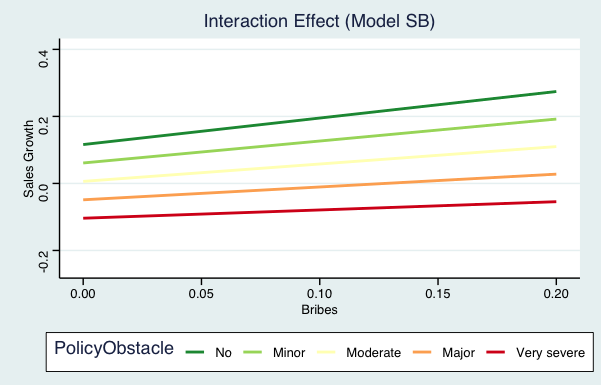
\includegraphics[scale=0.4]{chinchilab-template/Pictures/IE_ModelSB_a.png}
    \end{subfigure}
    \begin{subfigure}
    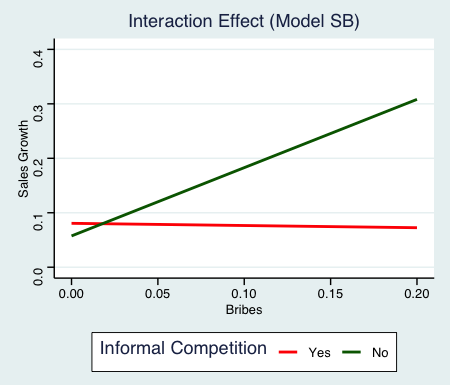
\includegraphics[scale=0.4]{chinchilab-template/Pictures/IE_ModelSB_b.png}
    \end{subfigure}
    \caption{Visualization of Interaction Effects in Model Employment Growth - Bribe Index}%
\end{figure}

%%%%%%%%%%%%%%%%%%%%%%%%%
\begin{landscape}
\thispagestyle{mylandscape}
\begin{table}[!htbp] \centering 
  \caption{Results of Model SB} 
  \label{} 
  \begin{adjustbox}{width=\columnwidth,center}
\begin{tabular}{@{\extracolsep{5pt}}lD{.}{.}{-3} D{.}{.}{-3} D{.}{.}{-3} D{.}{.}{-3} D{.}{.}{-3} D{.}{.}{-3} } 
\\[-1.8ex]\hline 
\hline \\[-1.8ex] 
 & \multicolumn{6}{c}{\textit{Dependent variable:}} \\ 
\cline{2-7} 
\\[-1.8ex] & \multicolumn{6}{c}{SalesGrowth} \\ 
\\[-1.8ex] & \multicolumn{1}{c}{(Baseline)} & \multicolumn{1}{c}{(1)} & \multicolumn{1}{c}{(2a)} & \multicolumn{1}{c}{(2b)} & \multicolumn{1}{c}{(3a)} & \multicolumn{1}{c}{(3b)}\\ 
\hline \\[-1.8ex] 
  Bribes &  & 0.357 & 0.617 & 0.793 & 0.379 & \cellcolor{yellow}1.254^{*} \\ 
  &  & (0.418) & (0.437) & (0.990) & (0.438) & (0.754) \\ 
  PolicyObstacle &  &  & \cellcolor{yellow}-0.058^{*} & -0.055 &  &  \\ 
  &  &  & (0.031) & (0.035) &  &  \\ 
  Bribes $\times$ PolicyObstacle &  &  &  & -0.136 &  &  \\ 
  &  &  &  & (0.687) &  &  \\ 
  InformalCompetition &  &  &  &  & -0.008 & 0.023 \\ 
  &  &  &  &  & (0.048) & (0.052) \\ 
  Bribes $\times$ InformalCompetition &  &  &  &  &  & -1.295 \\ 
  &  &  &  &  &  & (0.911) \\ 
 Sector & -0.083 & -0.084 & -0.085 & -0.086 & -0.083 & -0.084 \\ 
  & (0.052) & (0.053) & (0.052) & (0.053) & (0.053) & (0.053) \\ 
  Small & -0.026 & -0.024 & -0.023 & -0.025 & -0.021 & -0.016 \\ 
  & (0.061) & (0.061) & (0.060) & (0.061) & (0.064) & (0.064) \\ 
  Medium & -0.011 & -0.012 & -0.011 & -0.012 & -0.010 & -0.010 \\ 
  & (0.056) & (0.056) & (0.055) & (0.056) & (0.056) & (0.056) \\ 
  lnAge & -0.049 & -0.050 & -0.055 & -0.056 & -0.050 & -0.056 \\ 
  & (0.042) & (0.043) & (0.042) & (0.042) & (0.043) & (0.043) \\ 
  lnExperience & \cellcolor{yellow}0.128^{***} & \cellcolor{yellow}0.128^{***} & \cellcolor{yellow}0.126^{***} & \cellcolor{yellow}0.126^{***} & \cellcolor{yellow}0.129^{***} & \cellcolor{yellow}0.140^{***} \\ 
  & (0.045) & (0.045) & (0.045) & (0.045) & (0.045) & (0.046) \\ 
  Foreign & -0.017 & -0.011 & -0.005 & -0.007 & -0.010 & -0.028 \\ 
  & (0.086) & (0.087) & (0.086) & (0.087) & (0.087) & (0.087) \\ 
  Export & 0.058 & 0.055 & 0.075 & 0.077 & 0.054 & 0.057 \\ 
  & (0.072) & (0.072) & (0.073) & (0.073) & (0.073) & (0.073) \\ 
  TrainingEmployees & \cellcolor{yellow}-0.120^{***} & \cellcolor{yellow}-0.126^{***} & \cellcolor{yellow}-0.127^{***} & \cellcolor{yellow}-0.128^{***} & \cellcolor{yellow}-0.126^{***} & \cellcolor{yellow}-0.121^{***} \\ 
  & (0.045) & (0.046) & (0.045) & (0.046) & (0.046) & (0.046) \\ 
  R\&D & \cellcolor{yellow}0.108^{**} & \cellcolor{yellow}0.118^{**} & \cellcolor{yellow}0.147^{***} & \cellcolor{yellow}0.147^{***} & \cellcolor{yellow}0.120^{**} & \cellcolor{yellow}0.112^{**} \\ 
  & (0.052) & (0.053) & (0.055) & (0.055) & (0.055) & (0.055) \\ 
  Constant & -0.114 & -0.121 & -0.064 & -0.066 & -0.122 & -0.155 \\ 
  & (0.142) & (0.142) & (0.144) & (0.145) & (0.143) & (0.144) \\ 
 \hline \\[-1.8ex] 
Observations & \multicolumn{1}{c}{160} & \multicolumn{1}{c}{160} & \multicolumn{1}{c}{160} & \multicolumn{1}{c}{160} & \multicolumn{1}{c}{160} & \multicolumn{1}{c}{160} \\ 
R$^{2}$ & \multicolumn{1}{c}{0.105} & \multicolumn{1}{c}{0.109} & \multicolumn{1}{c}{0.130} & \multicolumn{1}{c}{0.130} & \multicolumn{1}{c}{0.109} & \multicolumn{1}{c}{0.121} \\ 
Adjusted R$^{2}$ & \multicolumn{1}{c}{0.051} & \multicolumn{1}{c}{0.049} & \multicolumn{1}{c}{0.066} & \multicolumn{1}{c}{0.059} & \multicolumn{1}{c}{0.043} & \multicolumn{1}{c}{0.049} \\ 
Residual Std. Error & \multicolumn{1}{c}{0.261 (df = 150)} & \multicolumn{1}{c}{0.261 (df = 149)} & \multicolumn{1}{c}{0.259 (df = 148)} & \multicolumn{1}{c}{0.260 (df = 147)} & \multicolumn{1}{c}{0.262 (df = 148)} & \multicolumn{1}{c}{0.261 (df = 147)} \\ 
F Statistic & \multicolumn{1}{c}{1.946$^{**}$ (df = 9; 150)} & \multicolumn{1}{c}{1.821$^{*}$ (df = 10; 149)} & \multicolumn{1}{c}{2.015$^{**}$ (df = 11; 148)} & \multicolumn{1}{c}{1.838$^{**}$ (df = 12; 147)} & \multicolumn{1}{c}{1.648$^{*}$ (df = 11; 148)} & \multicolumn{1}{c}{1.689$^{*}$ (df = 12; 147)} \\ 
\hline 
\hline \\[-1.8ex] 
\textit{Note:}  & \multicolumn{6}{r}{$^{*}$p$<$0.1; $^{**}$p$<$0.05; $^{***}$p$<$0.01} \\ 
\end{tabular} 
\end{adjustbox}
\end{table} 
\end{landscape}
%%%%%%%%%%%%%%%%%%%%%%%%%

With regard to the control variables three of them show a significant effect on sales growth. First, manager experience has the expected positive sign and is significant with a p-value below 0.01. Second, employee training programs has an unexpected negative sign at the same significance level as the former. Third, R/&D has also an unexpected positive sign at the 5\% significance level. Lastly, the results of model SB are to a great extent in line with the outcomes of the labor productivity growth - bribes regressions. In particular the moderating effect of informal competition points towards the same direction and is significant even at the 10\% level. On the downside, the results of the employment growth - bribes regressions show a low predictive power. The only significant variable is policy obstacle. The coefficient's sign is in line with the results of the other models.

Next we present the results of bribe index as a proxy for administrative corruption. Unfortunately, bribe index seems to be a bad proxy in explaining the effect of corruption on firm growth. Nonetheless, we will present the employment growth - bribe index regressions depicted in \textbf{table 4.2} since they contain the most interpretable results. The regression in column 1 shows that bribe index has a positive effect on employment growth. This effect is insignificant in all regressions except for column 2b. By including the interaction effect of bribe index and policy obstacle, the coefficient of bribe index becomes significant (10\%). Moreover, the bribe index coefficient switched sign in the 
last regression when including the interaction effect with informal competition. We will come back to this but first,
Column 2a shows further validation of our hypothesis 2a with policy obstacle having a negative effect on firm performance. Next, \textbf{figure 4.2a} depicts the (insignificant) interaction effect of regression 2b. Due to relatively low standard errors the effect becomes more interpretable than the previous one in model SB. The graph visualizes that the positive effect of corruption on firm performance diminishes with increasing policy obstacle scores. Interestingly, the effect switches from positive to negative once firms experience policy obstacle to be major. Again, this is contrary to what we have hypothesized in hypothesis 2b.

\begin{figure}[h]%
    \centering
    \begin{subfigure}
    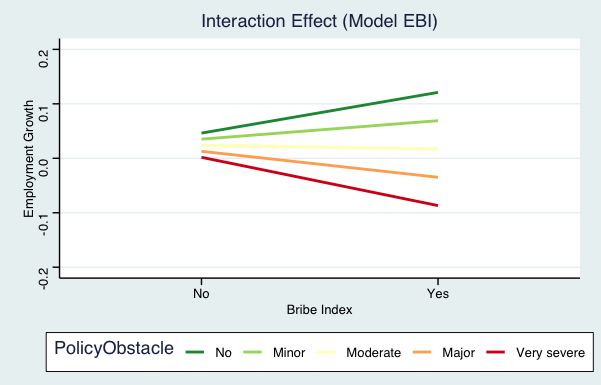
\includegraphics[scale=0.4]{chinchilab-template/Pictures/IE_ModelEBI_a.png}
    \end{subfigure}
    \begin{subfigure}
    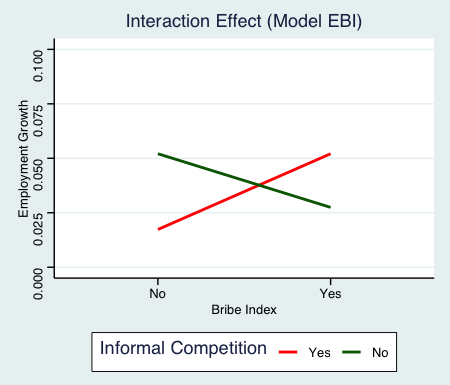
\includegraphics[scale=0.4]{chinchilab-template/Pictures/IE_ModelEBI_b.png}
    \end{subfigure}
    \caption{Visualization of Interaction Effects in Model Employment Growth - Bribe Index}%
\end{figure}

\begin{landscape}
\thispagestyle{mylandscape}
\begin{table}[!htbp] \centering 
  \caption{Results of Model EBI} 
  \label{} 
  \begin{adjustbox}{width=\columnwidth,center}
\begin{tabular}{@{\extracolsep{5pt}}lD{.}{.}{-3} D{.}{.}{-3} D{.}{.}{-3} D{.}{.}{-3} D{.}{.}{-3} D{.}{.}{-3} } 
\\[-1.8ex]\hline 
\hline \\[-1.8ex] 
 & \multicolumn{6}{c}{\textit{Dependent variable:}} \\ 
\cline{2-7} 
\\[-1.8ex] & \multicolumn{6}{c}{EmploymentGrowth} \\ 
\\[-1.8ex] & \multicolumn{1}{c}{(Baseline)} & \multicolumn{1}{c}{(1)} & \multicolumn{1}{c}{(2a)} & \multicolumn{1}{c}{(2b)} & \multicolumn{1}{c}{(3a)} & \multicolumn{1}{c}{(3b)}\\ 
\hline \\[-1.8ex] 
  BribeIndex &  & 0.004 & 0.016 & \cellcolor{yellow}0.075^{*} & 0.007 & -0.025 \\ 
  &  & (0.018) & (0.019) & (0.042) & (0.018) & (0.026) \\ 
  PolicyObstacle &  &  & \cellcolor{yellow}-0.018^{*} & -0.011 &  &  \\ 
  &  &  & (0.010) & (0.011) &  &  \\ 
  BribeIndex $\times$ PolicyObstacle &  &  &  & -0.041 &  &  \\ 
  &  &  &  & (0.026) &  &  \\ 
  InformalCompetition &  &  &  &  & -0.021 & \cellcolor{yellow}-0.035^{**} \\ 
  &  &  &  &  & (0.015) & (0.018) \\ 
  BribeIndex $\times$ InformalCompetition &  &  &  &  &  & \cellcolor{yellow}0.059^{*} \\ 
  &  &  &  &  &  & (0.036) \\ 
 Sector & -0.018 & -0.018 & -0.017 & -0.021 & -0.016 & -0.014 \\ 
  & (0.019) & (0.019) & (0.019) & (0.019) & (0.019) & (0.019) \\ 
  Small & -0.030 & -0.030 & -0.029 & -0.031 & -0.023 & -0.023 \\ 
  & (0.022) & (0.022) & (0.021) & (0.021) & (0.022) & (0.022) \\ 
  Medium & 0.007 & 0.007 & 0.006 & 0.003 & 0.009 & 0.007 \\ 
  & (0.020) & (0.020) & (0.020) & (0.020) & (0.020) & (0.020) \\ 
  lnAge & -0.012 & -0.013 & -0.014 & -0.015 & -0.012 & -0.008 \\ 
  & (0.015) & (0.015) & (0.015) & (0.015) & (0.015) & (0.015) \\ 
  lnExperience & \cellcolor{yellow}-0.027^{*} & \cellcolor{yellow}-0.028^{*} & \cellcolor{yellow}-0.029^{*} & \cellcolor{yellow}-0.030^{**} & \cellcolor{yellow}-0.026^{*} & \cellcolor{yellow}-0.030^{*} \\ 
  & (0.015) & (0.015) & (0.015) & (0.015) & (0.015) & (0.015) \\ 
  Foreign & -0.008 & -0.008 & -0.011 & -0.015 & -0.009 & -0.011 \\ 
  & (0.030) & (0.030) & (0.030) & (0.030) & (0.030) & (0.030) \\ 
  Export & 0.019 & 0.018 & 0.021 & 0.028 & 0.016 & 0.018 \\ 
  & (0.025) & (0.026) & (0.026) & (0.026) & (0.026) & (0.026) \\ 
  TrainingEmployees & 0.016 & 0.016 & 0.017 & 0.015 & 0.016 & 0.015 \\ 
  & (0.015) & (0.015) & (0.015) & (0.015) & (0.015) & (0.015) \\ 
  R\&D & 0.004 & 0.004 & 0.008 & 0.008 & 0.008 & 0.011 \\ 
  & (0.018) & (0.018) & (0.018) & (0.018) & (0.019) & (0.019) \\ 
  Constant & 0.154^{***} & 0.155^{***} & 0.178^{***} & 0.180^{***} & 0.154^{***} & 0.161^{***} \\ 
  & (0.049) & (0.049) & (0.050) & (0.050) & (0.049) & (0.049) \\ 
 \hline \\[-1.8ex] 
Observations & \multicolumn{1}{c}{255} & \multicolumn{1}{c}{255} & \multicolumn{1}{c}{255} & \multicolumn{1}{c}{255} & \multicolumn{1}{c}{255} & \multicolumn{1}{c}{255} \\ 
R$^{2}$ & \multicolumn{1}{c}{0.052} & \multicolumn{1}{c}{0.052} & \multicolumn{1}{c}{0.066} & \multicolumn{1}{c}{0.076} & \multicolumn{1}{c}{0.059} & \multicolumn{1}{c}{0.070} \\ 
Adjusted R$^{2}$ & \multicolumn{1}{c}{0.017} & \multicolumn{1}{c}{0.013} & \multicolumn{1}{c}{0.024} & \multicolumn{1}{c}{0.030} & \multicolumn{1}{c}{0.017} & \multicolumn{1}{c}{0.024} \\ 
Residual Std. Error & \multicolumn{1}{c}{0.116 (df = 245)} & \multicolumn{1}{c}{0.116 (df = 244)} & \multicolumn{1}{c}{0.116 (df = 243)} & \multicolumn{1}{c}{0.115 (df = 242)} & \multicolumn{1}{c}{0.116 (df = 243)} & \multicolumn{1}{c}{0.116 (df = 242)} \\ 
F Statistic & \multicolumn{1}{c}{1.494 (df = 9; 245)} & \multicolumn{1}{c}{1.345 (df = 10; 244)} & \multicolumn{1}{c}{1.558 (df = 11; 243)} & \multicolumn{1}{c}{1.648$^{*}$ (df = 12; 242)} & \multicolumn{1}{c}{1.392 (df = 11; 243)} & \multicolumn{1}{c}{1.514 (df = 12; 242)} \\ 
\hline 
\hline \\[-1.8ex] 
\textit{Note:}  & \multicolumn{6}{r}{$^{*}$p$<$0.1; $^{**}$p$<$0.05; $^{***}$p$<$0.01} \\ 
\end{tabular} 
\end{adjustbox}
\end{table} 
\end{landscape}

Column 3a points out that informal competition has a (insignificant) negative effect on employment growth. However, this effect becomes significant at the 95\% confidence level in the last regression. The interaction effect of informal competition and bribe index is visualized in \textbf{figure 4.2b}. The moderating effect is positive and significant (10\% level). Interestingly, as we already mentioned, the coefficient of bribe index becomes negative in this regression. This means that the effect of bribe index on employment growth is negative when informal competition is 0. This can also be observed in the graph. Moreover, the negative effect of bribe index on employment growth diminishes and becomes positive once enterprises experience threats from the informal sector.
Lastly, the graph suggests that firms competing against informal sector firms are better off if they bribe public officials than if they are not involved in administrative bribery. Considering the control variables we can observe that managerial experience is the only significant variable (10\% level). The coefficient's negative sign is contrary to what we expected and suggest that managers with more years of experience lead to less employment growth in Albanian firms.
In comparison to models SBI and PBI, the results of model EBI differ to a great extent. For instance, the bribe index coefficient in the other two models points towards a negative relationship with firm growth. Nevertheless, the only significant effect (10\% level) can be found in regression 3b of model PBI. It shows that informal competition negatively moderates the positive effect of bribe index (sign of coefficient flipped) on labor productivity growth. This is contrary to what was discovered in model EBI.

The third proxy is a particular type of administrative corruption, i.e. inspection bribe. We decided to analyze the employment growth - inspection bribe model. The outputs are summarized in \textbf{table 4.4}. First of all, we can not assess hypothesis 1 since inspection bribe has high standard errors and $R^2$ remained the same. Regression 2a provides further evidence in favor of our hypothesis 2a. The coefficient of policy obstacle is significantly (5\%) negative. Moreover, the significance improves to 1\% confidence when we include the interaction effect. 

\begin{figure}[h]%
    \centering
    \begin{subfigure}
    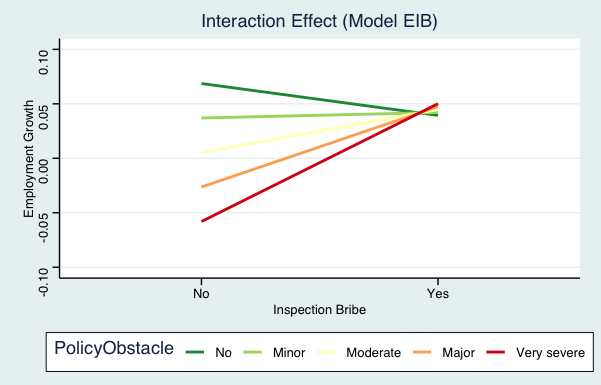
\includegraphics[scale=0.4]{chinchilab-template/Pictures/IE_ModelEIB_a.png}
    \end{subfigure}
    \begin{subfigure}
    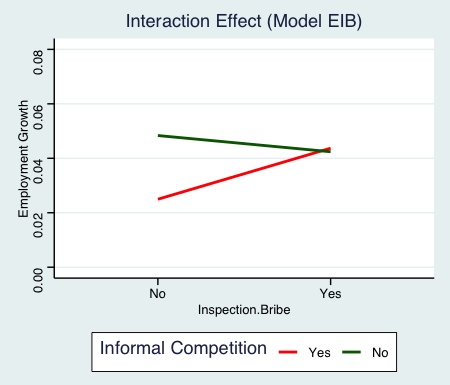
\includegraphics[scale=0.4]{chinchilab-template/Pictures/IE_ModelEIB_b.png}
    \end{subfigure}
    \caption{Visualization of Interaction Effects in Model Employment Growth - Bribe Index}%
\end{figure}

\begin{landscape}
\thispagestyle{mylandscape}
\begin{table}[!htbp] \centering 
  \caption{Results of Model EIB} 
  \label{} 
  \begin{adjustbox}{width=\columnwidth,center}
\begin{tabular}{@{\extracolsep{5pt}}lD{.}{.}{-3} D{.}{.}{-3} D{.}{.}{-3} D{.}{.}{-3} D{.}{.}{-3} D{.}{.}{-3} } 
\\[-1.8ex]\hline 
\hline \\[-1.8ex] 
 & \multicolumn{6}{c}{\textit{Dependent variable:}} \\ 
\cline{2-7} 
\\[-1.8ex] & \multicolumn{6}{c}{EmploymentGrowth} \\ 
\\[-1.8ex] & \multicolumn{1}{c}{(Baseline)} & \multicolumn{1}{c}{(1)} & \multicolumn{1}{c}{(2a)} & \multicolumn{1}{c}{(2b)} & \multicolumn{1}{c}{(3a)} & \multicolumn{1}{c}{(3b)}\\ 
\hline \\[-1.8ex] 
  Inspection.Bribe &  & 0.004 & 0.013 & -0.029 & 0.007 & -0.006 \\ 
  &  & (0.016) & (0.017) & (0.031) & (0.017) & (0.024) \\ 
  PolicyObstacle &  &  & \cellcolor{yellow}-0.020^{**} & \cellcolor{yellow}-0.032^{***} &  &  \\ 
  &  &  & (0.010) & (0.012) &  &  \\ 
  Inspection.Bribe $\times$ PolicyObstaclePolicyObstacle &  &  &  & 0.034 &  &  \\ 
  &  &  &  & (0.021) &  &  \\ 
  InformalCompetition &  &  &  &  & -0.015 & -0.023 \\ 
  &  &  &  &  & (0.016) & (0.020) \\ 
  Inspection.Bribe $\times$ InformalCompetition &  &  &  &  &  & 0.025 \\ 
  &  &  &  &  &  & (0.033) \\ 
 Sector & -0.008 & -0.008 & -0.007 & -0.002 & -0.007 & -0.007 \\ 
  & (0.019) & (0.020) & (0.019) & (0.020) & (0.020) & (0.020) \\ 
  Small & -0.032 & -0.032 & -0.033 & -0.033 & -0.028 & -0.029 \\ 
  & (0.022) & (0.022) & (0.022) & (0.022) & (0.023) & (0.023) \\ 
  Medium & 0.007 & 0.007 & 0.007 & 0.005 & 0.008 & 0.008 \\ 
  & (0.020) & (0.020) & (0.020) & (0.020) & (0.020) & (0.021) \\ 
  lnAge & -0.015 & -0.015 & -0.015 & -0.017 & -0.014 & -0.014 \\ 
  & (0.016) & (0.016) & (0.016) & (0.016) & (0.016) & (0.016) \\ 
  lnExperience & -0.023 & -0.023 & -0.025 & -0.023 & -0.022 & -0.023 \\ 
  & (0.016) & (0.016) & (0.016) & (0.016) & (0.016) & (0.016) \\ 
  Foreign & -0.008 & -0.007 & -0.009 & -0.008 & -0.008 & -0.008 \\ 
  & (0.032) & (0.032) & (0.032) & (0.032) & (0.032) & (0.032) \\ 
  Export & 0.006 & 0.006 & 0.010 & 0.005 & 0.005 & 0.005 \\ 
  & (0.026) & (0.026) & (0.026) & (0.026) & (0.026) & (0.026) \\ 
  TrainingEmployees & 0.021 & 0.021 & 0.022 & 0.025 & 0.021 & 0.019 \\ 
  & (0.016) & (0.016) & (0.016) & (0.016) & (0.016) & (0.016) \\ 
  R\&D & -0.002 & -0.001 & 0.005 & 0.007 & 0.003 & 0.005 \\ 
  & (0.018) & (0.019) & (0.019) & (0.019) & (0.019) & (0.020) \\ 
  Constant & 0.149^{***} & 0.148^{***} & 0.170^{***} & 0.182^{***} & 0.148^{***} & 0.152^{***} \\ 
  & (0.052) & (0.052) & (0.053) & (0.053) & (0.052) & (0.052) \\ 
 \hline \\[-1.8ex] 
Observations & \multicolumn{1}{c}{236} & \multicolumn{1}{c}{236} & \multicolumn{1}{c}{236} & \multicolumn{1}{c}{236} & \multicolumn{1}{c}{236} & \multicolumn{1}{c}{236} \\ 
R$^{2}$ & \multicolumn{1}{c}{0.050} & \multicolumn{1}{c}{0.050} & \multicolumn{1}{c}{0.067} & \multicolumn{1}{c}{0.079} & \multicolumn{1}{c}{0.054} & \multicolumn{1}{c}{0.056} \\ 
Adjusted R$^{2}$ & \multicolumn{1}{c}{0.012} & \multicolumn{1}{c}{0.008} & \multicolumn{1}{c}{0.022} & \multicolumn{1}{c}{0.029} & \multicolumn{1}{c}{0.007} & \multicolumn{1}{c}{0.005} \\ 
Residual Std. Error & \multicolumn{1}{c}{0.115 (df = 226)} & \multicolumn{1}{c}{0.115 (df = 225)} & \multicolumn{1}{c}{0.114 (df = 224)} & \multicolumn{1}{c}{0.114 (df = 223)} & \multicolumn{1}{c}{0.115 (df = 224)} & \multicolumn{1}{c}{0.115 (df = 223)} \\ 
F Statistic & \multicolumn{1}{c}{1.322 (df = 9; 226)} & \multicolumn{1}{c}{1.192 (df = 10; 225)} & \multicolumn{1}{c}{1.469 (df = 11; 224)} & \multicolumn{1}{c}{1.583$^{*}$ (df = 12; 223)} & \multicolumn{1}{c}{1.159 (df = 11; 224)} & \multicolumn{1}{c}{1.107 (df = 12; 223)} \\ 
\hline 
\hline \\[-1.8ex] 
\textit{Note:}  & \multicolumn{6}{r}{$^{*}$p$<$0.1; $^{**}$p$<$0.05; $^{***}$p$<$0.01} \\ 
\end{tabular} 
\end{adjustbox}
\end{table} 
\end{landscape}
Thus, the conditional effect of policy obstacle is even more negative when inspection bribe is 0. Similarly, although insignificant, the negative coefficient of inspection bribe suggests that if policy obstacle is 0 then firms bribing tax officials are worse of than firms which do not bribe. The interaction effect of regression 2b is visualized in \textbf{figure 4.3a}. Although insignificant, the positive moderating effect of policy obstacle points towards an indirect sanding effect. With increasing bureaucratic complexity the initial negative relationship between inspection bribe and sales growth improves and becomes positive. Moreover, this means that in an environment with high policy obstacles firms perform better if they grease the palms of tax inspectors. This would be in line with our hypothesis 2b. Next, the results of column 3a depict a negative though insignificant effect of informal competition on employment growth. The interaction effect of the last regression is depicted in \textbf{figure 4.3b}. It would suggest that informal competition positively moderates the initial negative effect of inspection bribe on employment growth. Lastly, all control variables are insignificant.

\subsection{Logit Regression Results}
Interpreting logistic regressions is cumbersome because it estimates conditional means in terms of logits (log odds; mathematically $log(\frac{p}{1-p})$). Computations into odd ratio or into probability are necessary to interpret the magnitude of the results. In other words: "how much likely are the results?" Since we are solely interested in the direction of the coefficients (i.e. less likely or more likely) we do not report our results with any transformations. Nonetheless, if necessary, the odd ratio can be calculated by exponentiating the log odds, i.e. $exp(coefficient)$, and the probability p can be calculated by applying the logistic function, i.e. $\frac{exp(coefficient)}{1+exp(coefficient)}$.

\textbf{Table 4.7} displays the regression results of the innovation index - bribe model. Hypothesis 1 is once more not testable because the standard errors of the bribe coefficient is too large. The insignificantly positive coefficient of policy obstacle in column 2a would suggest that for increasing values of policy obstacle firms are more likely to innovate. This would mean the opposite of our hypothesis 2a. Column 2b's interaction effect is visualized in \textbf{figure 4.4a}. Note that the y-axis is converted to a probability scale instead of a logit scale. Policy obstacle negatively moderates the relationship between bribes and innovation activities. This would conflict our hypothesis 2b. Regression 3a indicates that firms experiencing threats from the informal sector are less likely to innovate. In the last regression our corruption proxy becomes significant (10\% level), indicating that if firms do not experience informal competition they are more likely to innovate when bribing. The significant (10\% level) interaction effect of bribes and informal competition is visualized in \textbf{figure 4.4b}. The negative coefficient suggests that informal competition negatively moderates the relationship between bribes and innovation activities. Hence, the positive relationship between bribes and innovation activities becomes negative when firms encounter informal competition. This finding supports our hypothesis 3b. Lastly, five control variables show significance. First, firms operating in the manufacturing sector are more likely to innovate than firms operating in the service sector.  

\begin{landscape}
\thispagestyle{mylandscape}
\begin{table}[!htbp] \centering 
  \caption{Results of Model IB} 
  \label{} 
  \begin{adjustbox}{max width=\textwidth,center}
\begin{tabular}{@{\extracolsep{5pt}}lD{.}{.}{-3} D{.}{.}{-3} D{.}{.}{-3} D{.}{.}{-3} D{.}{.}{-3} D{.}{.}{-3} } 
\\[-1.8ex]\hline 
\hline \\[-1.8ex] 
 & \multicolumn{6}{c}{\textit{Dependent variable:}} \\ 
\cline{2-7} 
\\[-1.8ex] & \multicolumn{6}{c}{InnovationIndex} \\ 
\\[-1.8ex] & \multicolumn{1}{c}{(Baseline)} & \multicolumn{1}{c}{(1)} & \multicolumn{1}{c}{(2a)} & \multicolumn{1}{c}{(2b)} & \multicolumn{1}{c}{(3a)} & \multicolumn{1}{c}{(3b)}\\ 
\hline \\[-1.8ex] 
  Bribes &  & 1.010 & -0.517 & 5.064 & 2.011 & \cellcolor{yellow}9.810^{*} \\ 
  &  & (3.381) & (3.545) & (8.328) & (3.448) & (5.726) \\ 
  PolicyObstacle &  &  & 0.357 & \cellcolor{yellow}0.449^{*} &  &  \\ 
  &  &  & (0.242) & (0.271) &  &  \\ 
  Bribes $\times$ PolicyObstacle &  &  &  & -4.253 &  &  \\ 
  &  &  &  & (5.753) &  &  \\ 
  InformalCompetition &  &  &  &  & -0.464 & -0.110 \\ 
  &  &  &  &  & (0.365) & (0.412) \\ 
  Bribes $\times$ InformalCompetition &  &  &  &  &  & \cellcolor{yellow}-13.239^{*} \\ 
  &  &  &  &  &  & (7.313) \\ 
 Sector & \cellcolor{yellow}1.387^{***} & \cellcolor{yellow}1.388^{***} & \cellcolor{yellow}1.382^{***} & \cellcolor{yellow}1.334^{***} & \cellcolor{yellow}1.473^{***} & \cellcolor{yellow}1.476^{***} \\ 
  & (0.444) & (0.445) & (0.445) & (0.450) & (0.454) & (0.453) \\ 
  Small & -0.428 & -0.430 & -0.468 & -0.535 & -0.319 & -0.294 \\ 
  & (0.504) & (0.504) & (0.510) & (0.520) & (0.513) & (0.517) \\ 
  Medium & 0.711 & 0.711 & 0.713 & 0.664 & \cellcolor{yellow}0.777^{*} & \cellcolor{yellow}0.814^{*} \\ 
  & (0.454) & (0.454) & (0.457) & (0.463) & (0.459) & (0.467) \\ 
  lnAge & -0.316 & -0.325 & -0.313 & -0.324 & -0.308 & -0.331 \\ 
  & (0.271) & (0.273) & (0.274) & (0.275) & (0.273) & (0.276) \\ 
  lnExperience & -0.048 & -0.046 & -0.010 & 0.012 & -0.040 & 0.017 \\ 
  & (0.305) & (0.305) & (0.306) & (0.309) & (0.309) & (0.315) \\ 
  Foreign & 0.172 & 0.175 & 0.171 & 0.115 & 0.151 & -0.002 \\ 
  & (0.611) & (0.612) & (0.615) & (0.620) & (0.617) & (0.644) \\ 
  Export & \cellcolor{yellow}-1.416^{**} & \cellcolor{yellow}-1.424^{**} & \cellcolor{yellow}-1.562^{***} & \cellcolor{yellow}-1.520^{**} & \cellcolor{yellow}-1.479^{**} & \cellcolor{yellow}-1.455^{**} \\ 
  & (0.584) & (0.585) & (0.598) & (0.601) & (0.587) & (0.591) \\ 
  TrainingEmployees & \cellcolor{yellow}1.176^{***} & \cellcolor{yellow}1.159^{***} & \cellcolor{yellow}1.190^{***} & \cellcolor{yellow}1.175^{***} & \cellcolor{yellow}1.196^{***} & \cellcolor{yellow}1.278^{***} \\ 
  & (0.366) & (0.370) & (0.372) & (0.372) & (0.372) & (0.382) \\ 
  R\&D & -0.203 & -0.178 & -0.316 & -0.320 & -0.039 & -0.141 \\ 
  & (0.413) & (0.422) & (0.432) & (0.431) & (0.443) & (0.442) \\ 
  QualityCertificate & \cellcolor{yellow}0.822^{**} & \cellcolor{yellow}0.807^{**} & \cellcolor{yellow}0.853^{**} & \cellcolor{yellow}0.821^{**} & \cellcolor{yellow}0.768^{*} & \cellcolor{yellow}0.841^{**} \\ 
  & (0.399) & (0.402) & (0.406) & (0.409) & (0.403) & (0.413) \\ 
  Constant & -0.071 & -0.073 & -0.465 & -0.523 & -0.036 & -0.338 \\ 
  & (0.892) & (0.893) & (0.934) & (0.940) & (0.904) & (0.924) \\ 
 \hline \\[-1.8ex] 
Observations & \multicolumn{1}{c}{185} & \multicolumn{1}{c}{185} & \multicolumn{1}{c}{185} & \multicolumn{1}{c}{185} & \multicolumn{1}{c}{185} & \multicolumn{1}{c}{185} \\ 
Log Likelihood & \multicolumn{1}{c}{-108.995} & \multicolumn{1}{c}{-108.951} & \multicolumn{1}{c}{-107.839} & \multicolumn{1}{c}{-107.565} & \multicolumn{1}{c}{-108.136} & \multicolumn{1}{c}{-106.374} \\ 
Akaike Inf. Crit. & \multicolumn{1}{c}{239.990} & \multicolumn{1}{c}{241.902} & \multicolumn{1}{c}{241.678} & \multicolumn{1}{c}{243.129} & \multicolumn{1}{c}{242.272} & \multicolumn{1}{c}{240.748} \\ 
Pseudo R^{2} & \multicolumn{1}{c}{0.149} & \multicolumn{1}{c}{0.149} & \multicolumn{1}{c}{0.158} & \multicolumn{1}{c}{0.160} & \multicolumn{1}{c}{0.155} & \multicolumn{1}{c}{0.170} \\ 
\hline 
\hline \\[-1.8ex] 
\textit{Note:}  & \multicolumn{6}{r}{$^{*}$p$<$0.1; $^{**}$p$<$0.05; $^{***}$p$<$0.01} \\ 
\end{tabular} 
\end{adjustbox}
\end{table} 
\end{landscape}

Second, although only significant at the 10\% level in column 3a and 3b, medium sized enterprises (20-99 employ.) are more likely to innovate than large sized enterprises (100+ employ.). Third, firms exporting are less likely to innovate. Fourth, firms having a training program for their employees are more likely to innovate than firms which do have such training. Fifth, firms having a quality certificate are more likely to innovate than firms which do not have quality certificates.

\begin{figure}[h]%
    \centering
    \begin{subfigure}
    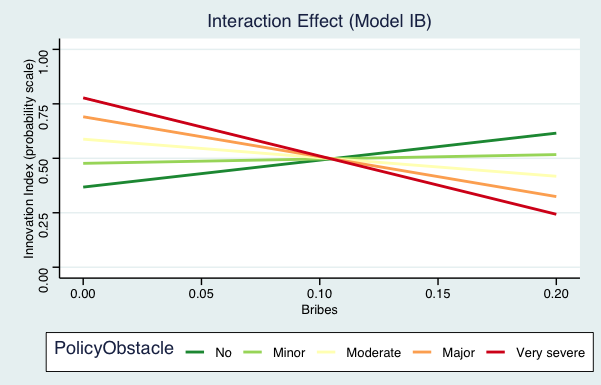
\includegraphics[scale=0.4]{chinchilab-template/Pictures/IE_ModelIB_a.png}
    \end{subfigure}
    \begin{subfigure}
    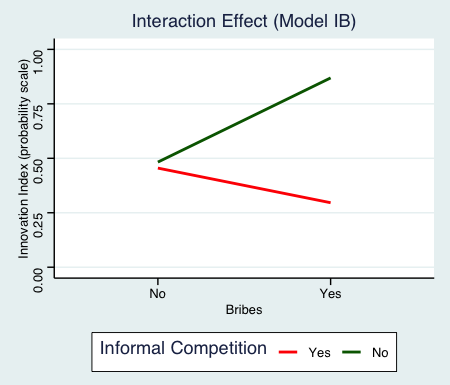
\includegraphics[scale=0.4]{chinchilab-template/Pictures/IE_ModelIB_b.png}
    \end{subfigure}
    \caption{Visualization of Interaction Effects in Model  Innovation Index - Bribes}%
\end{figure}

Next, we analyze the innovation index - bribe index model. The standard errors of our corruption proxy remains high. Nonetheless, the positive coefficient suggests that firms bribing at least in one of four administrative areas are more likely to innovate than firms which do not participate in these corrupt activities with public officials. Regression 2a reports a significantly (5\% level) positive policy obstacle coefficient which suggest that increasing levels of obstacles are related to firms being more likely to innovate. This represents further evidence in favor of hypothesis 2a.
Although the interaction effect of bribe index and policy obstacle suffers from high standard errors it can be visually assessed in \textbf{figure 4.5a}. The graph shows that policy obstacle negatively moderates the relationship of bribe index and innovation activities. This would imply evidence against hypothesis 2b. Next, the significantly (10\% level) negative coefficient of informal competition in regression 3a suggests that firms perceiving threats from informal firms are less likely to innovate. The interaction effect of the last regression is visualized in \textbf{figure 4.5b}. Unfortunately, the negative moderating effect of informal competition is not significant. Otherwise the results would be in line with hypothesis 3b. Lastly, the same five control variables as in the previous model are significant. Moreover, lnAge is significant at the 10\% confidence level indicating that older firms are less likely to innovate. 

\begin{landscape}
\thispagestyle{mylandscape}
\begin{table}[!htbp] \centering 
  \caption{Results of Model IBI} 
  \label{} 
  \begin{adjustbox}{max width=\textwidth,center}
\begin{tabular}{@{\extracolsep{5pt}}lD{.}{.}{-3} D{.}{.}{-3} D{.}{.}{-3} D{.}{.}{-3} D{.}{.}{-3} D{.}{.}{-3} } 
\\[-1.8ex]\hline 
\hline \\[-1.8ex] 
 & \multicolumn{6}{c}{\textit{Dependent variable:}} \\ 
\cline{2-7} 
\\[-1.8ex] & \multicolumn{6}{c}{InnovationIndex} \\ 
\\[-1.8ex] & \multicolumn{1}{c}{(Baseline)} & \multicolumn{1}{c}{(1)} & \multicolumn{1}{c}{(2a)} & \multicolumn{1}{c}{(2b)} & \multicolumn{1}{c}{(3a)} & \multicolumn{1}{c}{(3b)}\\ 
\hline \\[-1.8ex] 
 BribeIndex &  & 0.317 & 0.103 & 0.539 & 0.370 & 0.578 \\ 
  &  & (0.334) & (0.352) & (0.762) & (0.336) & (0.488) \\ 
  PolicyObstacle &  &  & \cellcolor{yellow}0.356^{**} & \cellcolor{yellow}0.409^{**} &  &  \\ 
  &  &  & (0.181) & (0.200) &  &  \\ 
  BribeIndex $\times$ PolicyObstacle &  &  &  & -0.308 &  &  \\ 
  &  &  &  & (0.475) &  &  \\ 
  InformalCompetition &  &  &  &  & \cellcolor{yellow}-0.479^{*} & -0.392 \\ 
  &  &  &  &  & (0.274) & (0.310) \\ 
  BribeIndex $\times$ InformalCompetition &  &  &  &  &  & -0.400 \\ 
  &  &  &  &  &  & (0.669) \\ 
  Sector & \cellcolor{yellow}1.387^{***} & \cellcolor{yellow}1.400^{***} & \cellcolor{yellow}1.381^{***} & \cellcolor{yellow}1.360^{***} & \cellcolor{yellow}1.445^{***} & \cellcolor{yellow}1.421^{***} \\ 
  & (0.360) & (0.362) & (0.364) & (0.365) & (0.365) & (0.365) \\ 
  Small & -0.483 & -0.490 & -0.532 & -0.553 & -0.381 & -0.371 \\ 
  & (0.402) & (0.403) & (0.407) & (0.408) & (0.410) & (0.410) \\ 
  Medium & \cellcolor{yellow}0.676^{*} & \cellcolor{yellow}0.656^{*} & \cellcolor{yellow}0.657^{*} & \cellcolor{yellow}0.641^{*} & \cellcolor{yellow}0.700^{*} & \cellcolor{yellow}0.721^{*} \\ 
  & (0.365) & (0.366) & (0.369) & (0.369) & (0.369) & (0.371) \\ 
  lnAge & \cellcolor{yellow}-0.391^{*} &\cellcolor{yellow} -0.418^{*} &\cellcolor{yellow} -0.406^{*} & \cellcolor{yellow}-0.399^{*} & \cellcolor{yellow}-0.407^{*} & \cellcolor{yellow}-0.421^{*} \\ 
  & (0.216) & (0.219) & (0.220) & (0.221) & (0.219) & (0.220) \\ 
  lnExperience & -0.061 & -0.058 & -0.043 & -0.050 & -0.031 & -0.016 \\ 
  & (0.228) & (0.229) & (0.231) & (0.231) & (0.230) & (0.232) \\ 
  Foreign & 0.102 & 0.067 & 0.134 & 0.099 & 0.034 & 0.038 \\ 
  & (0.489) & (0.492) & (0.496) & (0.501) & (0.496) & (0.501) \\ 
  Export & \cellcolor{yellow}-1.271^{***} & \cellcolor{yellow}-1.347^{***} & \cellcolor{yellow}-1.419^{***} & \cellcolor{yellow}-1.372^{***} & \cellcolor{yellow}-1.381^{***} & \cellcolor{yellow}-1.369^{***} \\ 
  & (0.476) & (0.486) & (0.493) & (0.496) & (0.487) & (0.487) \\ 
  TrainingEmployees & \cellcolor{yellow}1.047^{***} & \cellcolor{yellow}1.028^{***} & \cellcolor{yellow}1.076^{***} & \cellcolor{yellow}1.066^{***} & \cellcolor{yellow}1.033^{***} & \cellcolor{yellow}1.036^{***} \\ 
  & (0.278) & (0.279) & (0.282) & (0.283) & (0.281) & (0.281) \\ 
  R\&D & -0.296 & -0.284 & -0.335 & -0.333 & -0.178 & -0.192 \\ 
  & (0.333) & (0.334) & (0.336) & (0.335) & (0.345) & (0.345) \\ 
  QualityCertificate & \cellcolor{yellow}0.545^{*} & \cellcolor{yellow}0.557^{*} & \cellcolor{yellow}0.555^{*} & \cellcolor{yellow}0.557^{*} & \cellcolor{yellow}0.573^{*} & \cellcolor{yellow}0.596^{*} \\ 
  & (0.325) & (0.326) & (0.327) & (0.327) & (0.327) & (0.330) \\ 
  Constant & 0.532 & 0.551 & 0.165 & 0.133 & 0.576 & 0.518 \\ 
  & (0.723) & (0.725) & (0.754) & (0.755) & (0.730) & (0.736) \\ 
 \hline \\[-1.8ex] 
Observations & \multicolumn{1}{c}{289} & \multicolumn{1}{c}{289} & \multicolumn{1}{c}{289} & \multicolumn{1}{c}{289} & \multicolumn{1}{c}{289} & \multicolumn{1}{c}{289} \\ 
Log Likelihood & \multicolumn{1}{c}{-173.277} & \multicolumn{1}{c}{-172.824} & \multicolumn{1}{c}{-170.831} & \multicolumn{1}{c}{-170.620} & \multicolumn{1}{c}{-171.287} & \multicolumn{1}{c}{-171.107} \\ 
Akaike Inf. Crit. & \multicolumn{1}{c}{368.555} & \multicolumn{1}{c}{369.647} & \multicolumn{1}{c}{367.662} & \multicolumn{1}{c}{369.240} & \multicolumn{1}{c}{368.574} & \multicolumn{1}{c}{370.215} \\ 
Pseudo R^{2} & \multicolumn{1}{c}{0.131} & \multicolumn{1}{c}{0.133} & \multicolumn{1}{c}{0.143} & \multicolumn{1}{c}{0.144} & \multicolumn{1}{c}{0.141} & \multicolumn{1}{c}{0.142} \\ 
\hline 
\hline \\[-1.8ex] 
\textit{Note:}  & \multicolumn{6}{r}{$^{*}$p$<$0.1; $^{**}$p$<$0.05; $^{***}$p$<$0.01} \\ 
\end{tabular} 
\end{adjustbox}
\end{table} 
\end{landscape}

\begin{figure}[h]%
    \centering
    \begin{subfigure}
    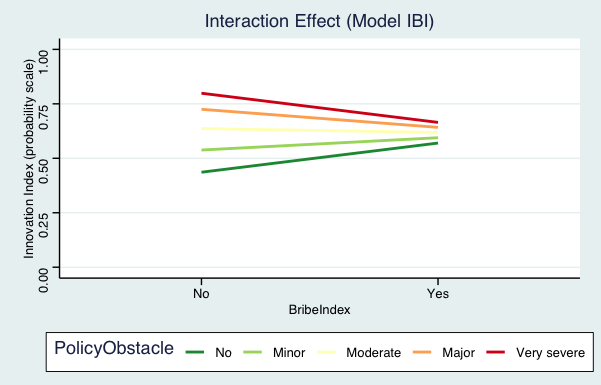
\includegraphics[scale=0.4]{chinchilab-template/Pictures/IE_ModelIBI_a.png}
    \end{subfigure}
    \begin{subfigure}
    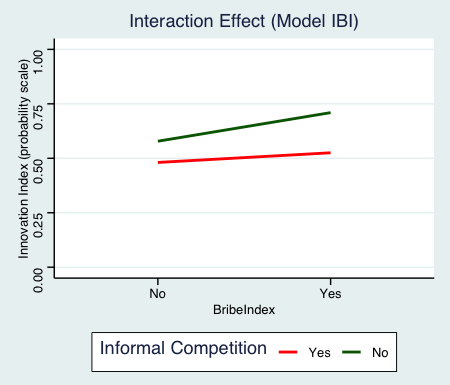
\includegraphics[scale=0.4]{chinchilab-template/Pictures/IE_ModelIBI_b.png}
    \end{subfigure}
    \caption{Visualization of Interaction Effects in Model Innovation Index - Bribe Index}%
\end{figure}

Finally, the innovation index - inspection bribe model is the last model presented in this study. In regression 1 we can observe that firm's bribing tax officials are more likely to innovate. Yet, this greasing effect is not significant. Regression 2a suggests that with increasing policy obstacle values Albanian firms are more likely to be an innovator. This effect is insignificant at a p value of 0.14 and would suggest the opposite of hypothesis 2a. Including the interaction effect in regression 2b yields a significant positive moderating effect (10\% level). The interaction effect of inspection bribe and policy obstacle can be exhibited in \textbf{figure 4.6a}. This greasing effect means that as the level of policy obstacle increases, the relationship between inspection bribe and firm innovation flips from a sanding to a greasing effect. Thus, firms bribing in an environment which is perceived having moderate, major or very severe policy obstacles are increasingly more likely to innovate. This provides evidence for our hypothesis 2b. 

\begin{figure}[h]%
    \centering
    \begin{subfigure}
    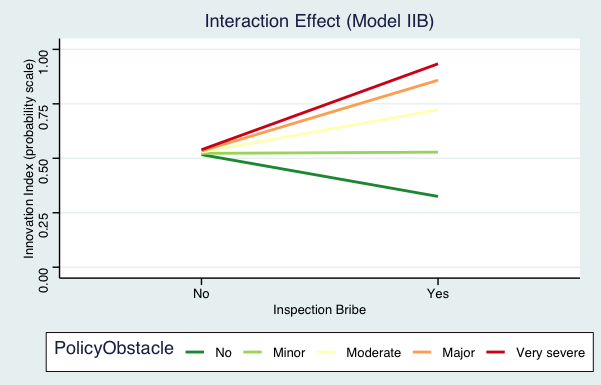
\includegraphics[scale=0.4]{chinchilab-template/Pictures/IE_ModelIIB_a.png}
    \end{subfigure}
    \begin{subfigure}
    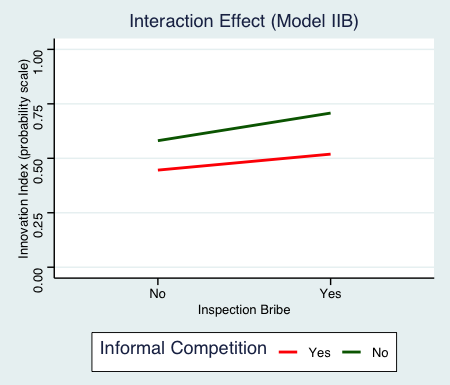
\includegraphics[scale=0.4]{chinchilab-template/Pictures/IE_ModelIIB_b.png}
    \end{subfigure}
    \caption{Visualization of Interaction Effects in Model Innovation Index - Inspection Bribe}%
\end{figure}

\begin{landscape}
\thispagestyle{mylandscape}
\begin{table}[!htbp] \centering 
  \caption{Results of Model IIB} 
  \label{} 
  \begin{adjustbox}{max width=\textwidth,center}
\begin{tabular}{@{\extracolsep{5pt}}lD{.}{.}{-3} D{.}{.}{-3} D{.}{.}{-3} D{.}{.}{-3} D{.}{.}{-3} D{.}{.}{-3} } 
\\[-1.8ex]\hline 
\hline \\[-1.8ex] 
 & \multicolumn{6}{c}{\textit{Dependent variable:}} \\ 
\cline{2-7} 
\\[-1.8ex] & \multicolumn{6}{c}{InnovationIndex} \\ 
\\[-1.8ex] & \multicolumn{1}{c}{(1)} & \multicolumn{1}{c}{(2)} & \multicolumn{1}{c}{(3)} & \multicolumn{1}{c}{(4)} & \multicolumn{1}{c}{(5)} & \multicolumn{1}{c}{(6)}\\ 
\hline \\[-1.8ex] 
 Inspection.Bribe &  & 0.343 & 0.207 & -0.782 & 0.437 & 0.555 \\ 
  &  & (0.299) & (0.312) & (0.601) & (0.306) & (0.435) \\ 
  PolicyObstacle &  &  & 0.284 & 0.039 &  &  \\ 
  &  &  & (0.184) & (0.221) &  &  \\ 
  Inspection.Bribe $\times$ PolicyObstacle &  &  &  & \cellcolor{yellow}0.808^{*} &  &  \\ 
  &  &  &  & (0.420) &  &  \\ 
  InformalCompetition &  &  &  &  & \cellcolor{yellow}-0.647^{**} & -0.568 \\ 
  &  &  &  &  & (0.289) & (0.353) \\ 
  Inspection.Bribe $\times$ InformalCompetition &  &  &  &  &  & -0.237 \\ 
  &  &  &  &  &  & (0.615) \\ 
  Sector & \cellcolor{yellow}1.488^{***} & \cellcolor{yellow}1.454^{***} & \cellcolor{yellow}1.451^{***} & \cellcolor{yellow}1.587^{***} & \cellcolor{yellow}1.520^{***} & \cellcolor{yellow}1.518^{***} \\ 
  & (0.379) & (0.381) & (0.383) & (0.397) & (0.385) & (0.384) \\ 
  Small & -0.505 & -0.517 & -0.530 & -0.497 & -0.402 & -0.391 \\ 
  & (0.422) & (0.424) & (0.425) & (0.430) & (0.431) & (0.432) \\ 
  Medium & 0.563 & 0.530 & 0.540 & 0.515 & 0.570 & 0.580 \\ 
  & (0.381) & (0.382) & (0.383) & (0.387) & (0.386) & (0.388) \\ 
  lnAge & \cellcolor{yellow}-0.367^{*} & -0.357 & -0.363 & \cellcolor{yellow}-0.395^{*} & -0.344 & -0.342 \\ 
  & (0.221) & (0.221) & (0.222) & (0.224) & (0.221) & (0.221) \\ 
  lnExperience & -0.163 & -0.190 & -0.166 & -0.172 & -0.161 & -0.160 \\ 
  & (0.236) & (0.238) & (0.241) & (0.242) & (0.241) & (0.241) \\ 
  Foreign & 0.028 & 0.065 & 0.102 & 0.151 & 0.004 & 0.007 \\ 
  & (0.539) & (0.541) & (0.546) & (0.547) & (0.545) & (0.547) \\ 
  Export & \cellcolor{yellow}-1.241^{**} & \cellcolor{yellow}-1.225^{**} & \cellcolor{yellow}-1.308^{**} & \cellcolor{yellow}-1.450^{***} & \cellcolor{yellow}-1.271^{**} & \cellcolor{yellow}-1.268^{**} \\ 
  & (0.499) & (0.501) & (0.509) & (0.526) & (0.503) & (0.503) \\ 
  TrainingEmployees & \cellcolor{yellow}1.116^{***} & \cellcolor{yellow}1.112^{***} & \cellcolor{yellow}1.136^{***} & \cellcolor{yellow}1.199^{***} & \cellcolor{yellow}1.119^{***} & \cellcolor{yellow}1.129^{***} \\ 
  & (0.290) & (0.291) & (0.293) & (0.299) & (0.295) & (0.296) \\ 
  R\&D & -0.287 & -0.202 & -0.264 & -0.232 & -0.034 & -0.058 \\ 
  & (0.337) & (0.346) & (0.348) & (0.353) & (0.362) & (0.367) \\ 
  QualityCertificate & 0.421 & 0.413 & 0.423 & 0.495 & 0.426 & 0.447 \\ 
  & (0.340) & (0.342) & (0.342) & (0.348) & (0.344) & (0.349) \\ 
  Constant & 0.740 & 0.686 & 0.389 & 0.638 & 0.740 & 0.690 \\ 
  & (0.758) & (0.762) & (0.786) & (0.800) & (0.772) & (0.782) \\ 
 \hline \\[-1.8ex] 
Observations & \multicolumn{1}{c}{268} & \multicolumn{1}{c}{268} & \multicolumn{1}{c}{268} & \multicolumn{1}{c}{268} & \multicolumn{1}{c}{268} & \multicolumn{1}{c}{268} \\ 
Log Likelihood & \multicolumn{1}{c}{-161.009} & \multicolumn{1}{c}{-160.346} & \multicolumn{1}{c}{-159.128} & \multicolumn{1}{c}{-157.180} & \multicolumn{1}{c}{-157.792} & \multicolumn{1}{c}{-157.718} \\ 
Akaike Inf. Crit. & \multicolumn{1}{c}{344.017} & \multicolumn{1}{c}{344.692} & \multicolumn{1}{c}{344.255} & \multicolumn{1}{c}{342.361} & \multicolumn{1}{c}{341.585} & \multicolumn{1}{c}{343.436} \\ 
Pseudo R^{2} & \multicolumn{1}{c}{0.129} & \multicolumn{1}{c}{0.133} & \multicolumn{1}{c}{0.139} & \multicolumn{1}{c}{0.150} & \multicolumn{1}{c}{0.146} & \multicolumn{1}{c}{0.147} \\ 
\hline 
\hline \\[-1.8ex] 
\textit{Note:}  & \multicolumn{6}{r}{$^{*}$p$<$0.1; $^{**}$p$<$0.05; $^{***}$p$<$0.01} \\ 
\end{tabular} 
\end{adjustbox}
\end{table} 
\end{landscape}

Next, the significant negative coefficient of informal competition in model 3a provides evidence in favor of hypothesis 3a. Finally, the interaction effect of inspection bribe and informal competition from the last regression has too high standard errors to be correctly interpretable. Nonetheless, the negative coefficient suggests a negative moderating effect which means that the positive relationship between inspection bribe and innovation activity is decreased by the occurrence of informal competition. Though, the magnitude of this moderating effect is low (almost parallel lines).

To summarize, the results of the presented models are mixed and partially confirm some of our hypotheses at a statistical significance ranging between 5-10\%. The first hypothesis is statistically not significant but the corruption coefficient's aim more or less in all models towards a positive relationship with firm performance. Nonetheless, the null hypothesis for the respective coefficients can not be rejected. Hypothesis 2a is statistically significant in all of the presented firm growth models. By contrast, the innovation models point towards a positive relationship with innovation activity. In particular, model IBI evinced a significant positive policy obstacle coefficient. Thus, hypothesis 2a is in line with the presented firm growth models but not with the innovation models. The regression results of equation 2b did not show the hypothesized moderating effect of policy obstacle except for the last presented model, which proxied firm performance as innovation activity and corruption as tax inspection bribe. Next, the penultimate hypothesis was found to be partially significant. More precisely, models EBI, IBI and IIB showed significant negative effects of informal competition on firm performance. Although insignificant, the effect of informal competition on firm performance was negative in all of the other presented models. Considering the last hypothesis we found mixed results in the firm growth models. Model EBI was the only model which revealed a significant positive moderating effect, though this is contrary to what we have hypothesized. Moreover, the innovation models IBI and IIB showed the expected effect whereby informal competition exerts a significantly negative moderating effect on the relationship between corruption and firm performance. These results will be further discussed in the next chapter.